\definecolor{red}{rgb}{0.827,0.196,0.122}
\definecolor{orange}{rgb}{1.0,0.498,0.0}
\definecolor{olive}{rgb}{0.71,0.71,0.345}
\definecolor{green}{rgb}{0.118,0.490,0.216}
\definecolor{blue}{rgb}{0.447,0.624,0.812}

\chapter{Entwurf}
\label{chapter:design}
    Nachdem im vorangegangenem Kapitel die Anforderungen für das System spezifiziert wurden, sollen in diesem Kapitel die Überlegungen zum Design der verschiedenen Sichten dargestellt werden.
    
    \section{Datenmodell}
    
    \section{Design}
        Für den Desing-Entwurf der Seite wurden Mock-Ups erstellt, die den groben Aufbau der Website mit den entsprechenden Funktionen zeigt. 
        Im folgenden werden diese Mock-Ups für das sogenannte Frontend, also aus Sicht der Studenten, und für das Backend, die Sicht der Dozenten beziehungsweise der Administratoren, vorgestellt.
        Dabei gilt der in Tabelle \ref{tab:Farbcode} angegebene Farbcode für die verschiedenen Elemente der Mock-Ups.
        \begin{table}
            \centering
            \begin{tabular}{l c| l}
                \cellcolor{red} & & Eingabefeld\\\\
                \cellcolor{orange} & & Button\\\\
                \cellcolor{olive} & & Drag\&Drop-Element\\\\
                \cellcolor{green} & & Textfeld\\\\
                \cellcolor{blue} & & Optisches Element
            \end{tabular}
            \caption{Farbcode der Mock-Ups}
            \label{tab:Farbcode}
        \end{table}
    
        \subsection{Frontend}
            Wie in Kapitel \ref{chapter:requirements} bereits ausgeführt, sollen die Studenten zunächst eine Registrierungs- bzw. Login-Oberfläche sehen.
            Jedoch sollen die verschiedenen Kurse auch ohne eine Anmeldung einsehbar sein.
            \begin{figure}[t]
            	\centering
            	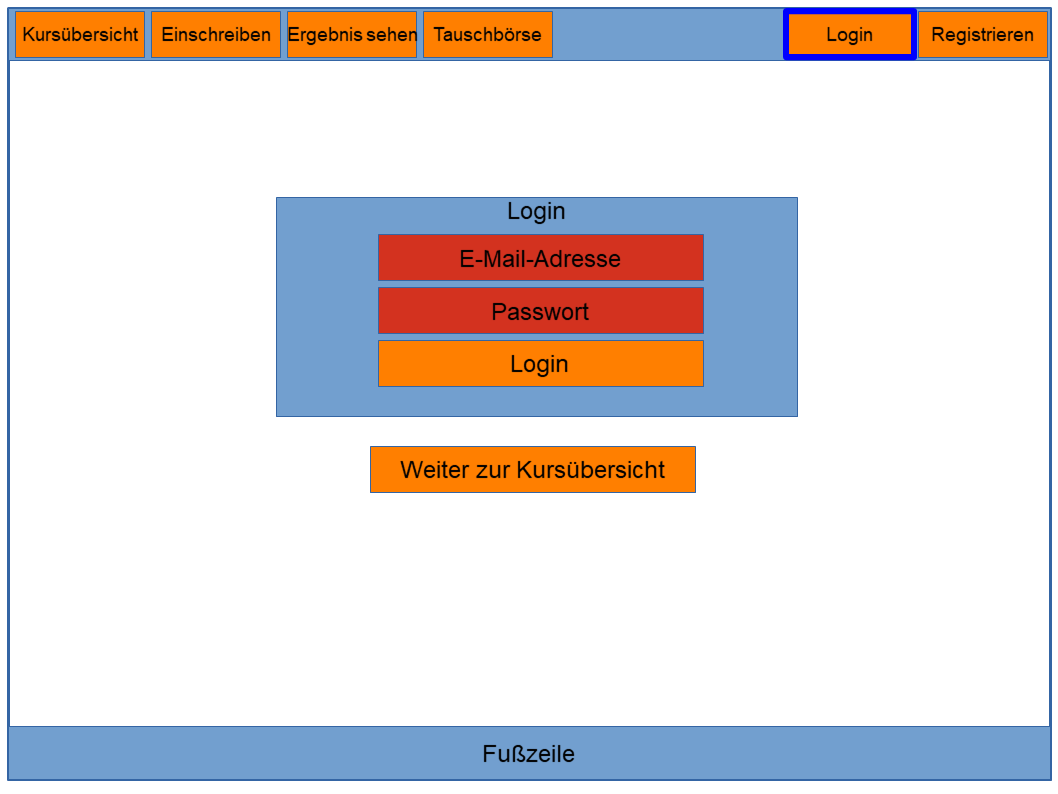
\includegraphics[width=0.7\textwidth]{./design/MockUpsFrontend/frontendLogin.png}
            	\caption{Entwurf für die Login-Oberfläche}
            	\label{mockupLoginFrontend}
            \end{figure}   
        
            In Abbildung \ref{mockupLoginFrontend} werden beide Anforderungen umgesetzt.
            Zum einen die Login-Oberfläche, in der in zwei Textfelder Benutzername und Passwort für einen erfolgreichen Login eingetragen werden müssen, zum anderen die direkte Weiterleitung zur Kursübersicht als einfacher Knopf darunter.

            Die Kopfzeile umfasst einige Reiter.
            So kann mithilfe der Kopfzeile auf die verschiedenen Funktionen des Frontends gewechselt werden. 
            Dazu zählen die Kursübersicht, die Erstellung der Präferenzliste, das Einsehen der Verteilungsergebnisse, sowie das Tauschen von Kursen.
            Außerdem soll in der Kopfzeile ein Schalter zum Abmelden aus dem System bereitgestellt werden und eine Anzeige, ab wann das Ende der Einschreibungs- und Tauschphase erreicht ist.
            Auf allen weiteren Seiten soll die Kopfzeile die gleiche Funktion und das gleiche Aussehen haben.
            Unter der Kopfzeile folgt eine textuelle Erklärung des Ablaufs des Empiriepraktikums und der für die Studenten relevanten Schritte, um sich erfolgreich für die Kurse einzuschreiben.
            Wie in Abbildung \ref{mockupCoursesFrontend} dargestellt, werden darunter die verschiedenen Kurse angezeigt, jeweils mit einer kurzen Beschreibung.
            Durch einen Klick auf ein Kursfeld, sollen sich die detaillierten Informationen zu dem Kurs einsehen lassen.
            Das Desing hierfür ist in Abbildung \ref{mockupDetailsFrontend} zu sehen und bedarf keiner weiteren Erläuterung.
            \begin{figure}[t]
            	\centering
            	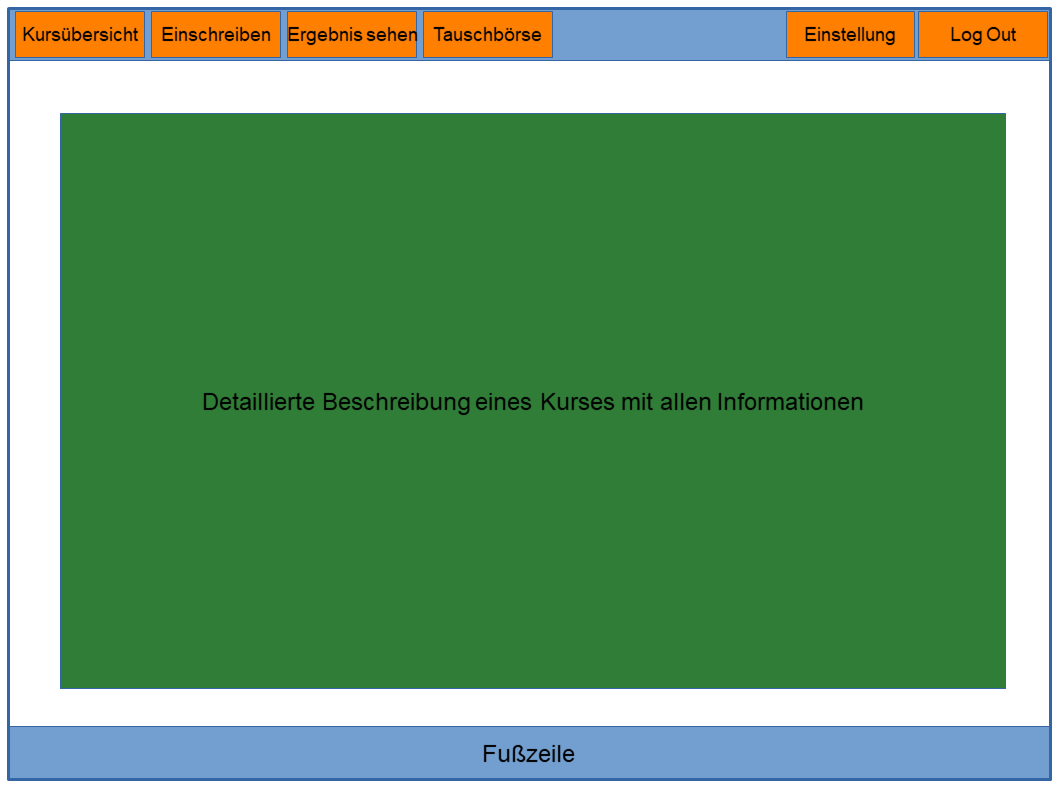
\includegraphics[width=0.7\textwidth]{./design/MockUpsFrontend/frontendCoursedetails.png}
            	\caption{Entwurf für die Kursdetails}
            	\label{mockupDetailsFrontend}
            \end{figure}
            Die Fußzeile soll weitere allgemeine Informationen bereitstellen, sofern diese von Nöten sein sollten, aber vor allem als optischer Abschluss der Seite dienen.
            \begin{figure}[t]
            	\centering
            	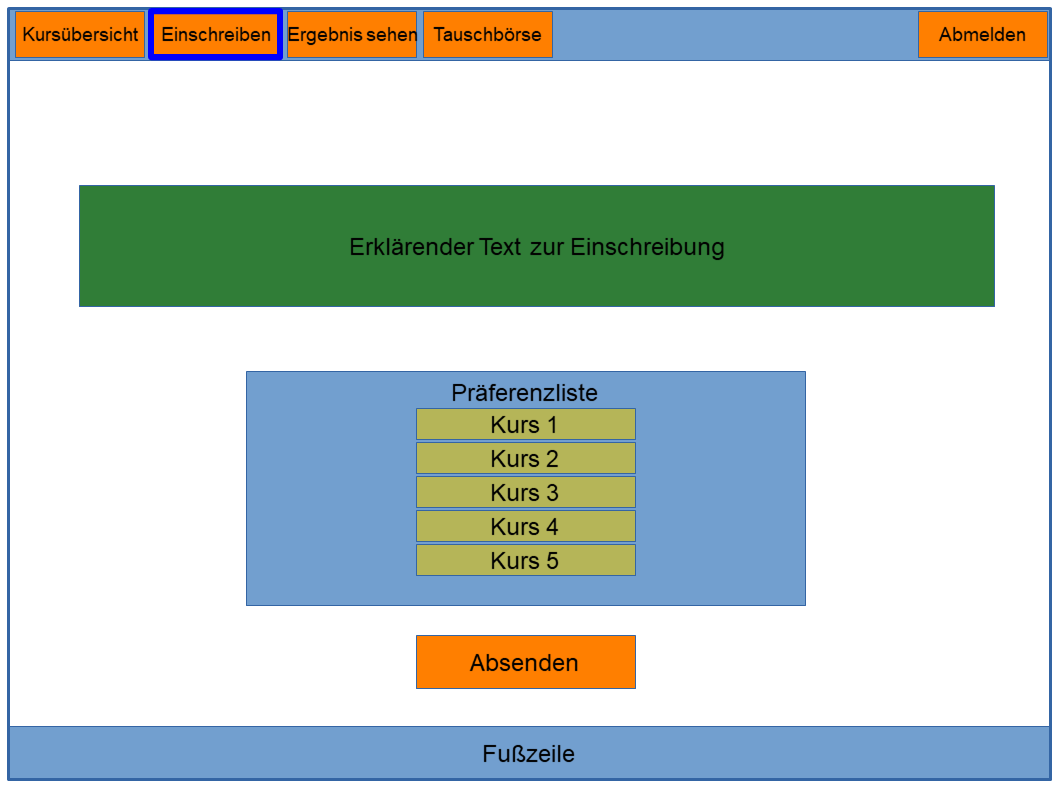
\includegraphics[width=0.7\textwidth]{./design/MockUpsFrontend/frontendPreferences.png}
            	\caption{Entwurf für die Einschreibungs-Oberfläche}
            	\label{mockupPreferencesFrontend}
            \end{figure}
            
            Die Seite für die Einschreibung in die Kurse soll wie in Abbildung \ref{mockupPreferencesFrontend} gestaltet sein.
            Wieder bilden Kopfzeile und Fußzeile den Rahmen der Seite.
            Unter der Kopfzeile befindet sich auch hier eine kurze Erklärung, wie man die Präferenzliste genau erstellt.
            Das Erstellen soll im Feld \textit{Präferenzliste} über ein ''Drag\&Drop''-System vorgenommen werden und über den Knopf \textit{Absenden} fixiert werden können.
            
            \begin{figure}[t]
                \centering
                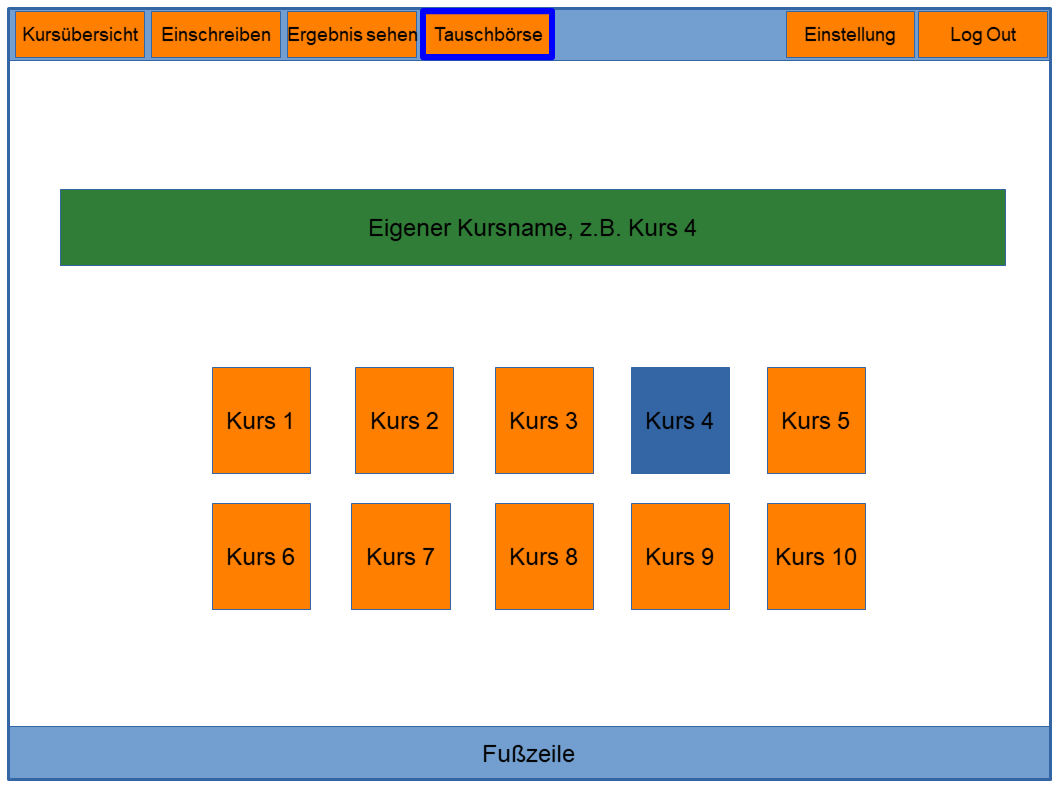
\includegraphics[width=0.7\textwidth]{./design/MockUpsFrontend/frontendSwap1.png}
                \caption{Entwurf für die Tauschauswahl}
                \label{mockupResultsFrontend}
            \end{figure}
        
            \begin{figure}[t]
                \centering
                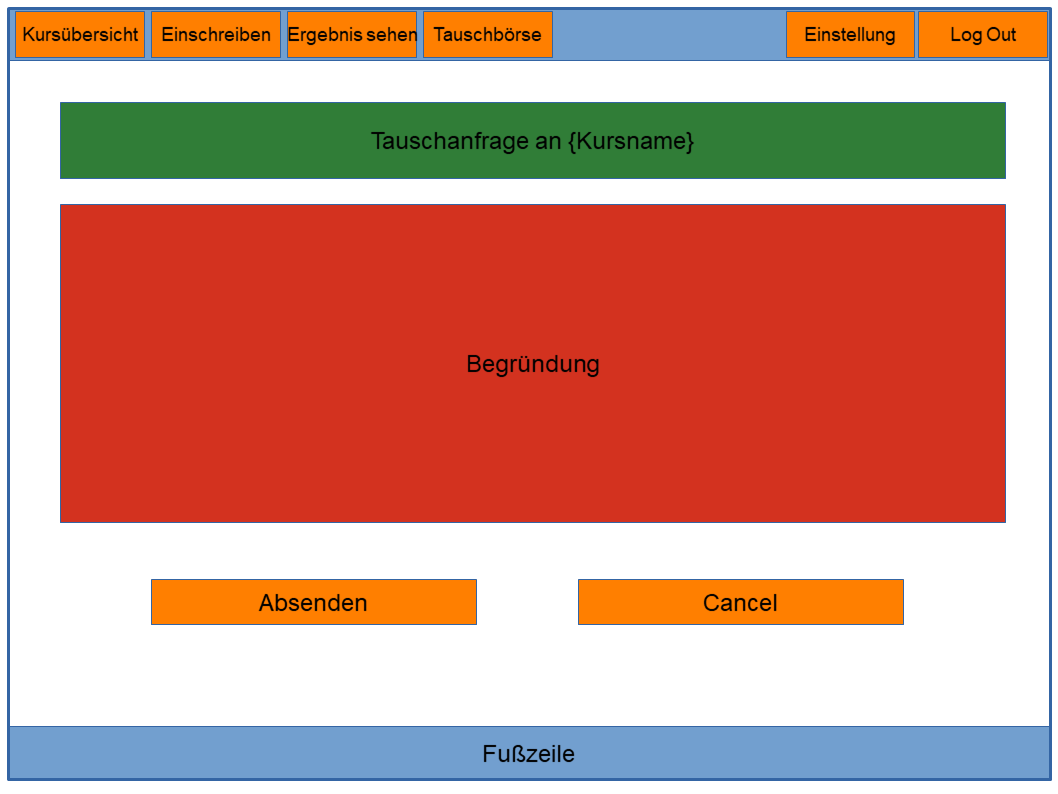
\includegraphics[width=0.7\textwidth]{./design/MockUpsFrontend/frontendSwap2.png}
                \caption{Entwurf für die Tauschanfrage}
                \label{mockupResultsFrontend}
            \end{figure}
            
    
        \subsection{Backend}
        	\subsubsection{Administratoren}
        	\subsubsection{Dozenten}